%++++++++++++++++++++++++++++++++++++++++
\documentclass[article, 12pt]{article}
\usepackage{float}
\usepackage{setspace}
\usepackage{tabu} % extra features for tabular environment
\usepackage{amsmath}  % improve math presentation
\usepackage{graphicx} % takes care of graphic including machinery
\usepackage[margin=1in]{geometry} % decreases margins
\usepackage{cite} % takes care of citations
\usepackage[final]{hyperref} % adds hyper links inside the generated pdf file
\usepackage{tikz}
\usepackage{caption} 
\usepackage{fancyhdr}
\usepackage{amssymb} % symbols like /therefore
\usepackage{amsthm} % proofs
\usepackage{enumerate} % lettered lists
\usepackage{mathtools} % macros 
\usepackage{tkz-graph}
\usepackage{tikz-layers}
\usepackage[colour, all, curve, arc, frame]{xy} % for diagrams
\usetikzlibrary{scopes}
\usetikzlibrary{graphs,graphs.standard,calc}
% \usepackage{xcolor} \pagecolor[rgb]{0.12549019607,0.1294117647,0.13725490196} \color[rgb]{0.82352941176,0.76862745098,0.62745098039} % dark theme
\theoremstyle{definition}
\newtheorem{example}{Example}[subsubsection]
\newtheorem*{remark}{Remark}
\newtheorem{theorem}{Theorem}[subsubsection]
\newtheorem{definition}{Definition}[subsubsection]
\newtheorem{corollary}{Corollary}[subsubsection]
\hypersetup{
	colorlinks=false,      % false: boxed links; true: colored links
	linkcolor=blue,        % color of internal links
	citecolor=blue,        % color of links to bibliography
	filecolor=magenta,     % color of file links
	urlcolor=blue         
}
\usepackage{physics}
\usepackage{siunitx}
\usepackage{tikz,pgfplots}
\usepackage[outline]{contour} % glow around text
\usetikzlibrary{calc}
\usetikzlibrary{angles,quotes} % for pic
\usetikzlibrary{arrows.meta}
\usetikzlibrary{automata}
\usetikzlibrary{arrows.meta, automata, positioning, quotes}
\tikzset{>=latex} % for LaTeX arrow head
\contourlength{1.2pt}

\colorlet{xcol}{blue!70!black}
\colorlet{vcol}{green!60!black}
\colorlet{myred}{red!70!black}
\colorlet{myblue}{blue!70!black}
\colorlet{mygreen}{green!70!black}
\colorlet{mydarkred}{myred!70!black}
\colorlet{mydarkblue}{myblue!60!black}
\colorlet{mydarkgreen}{mygreen!60!black}
\colorlet{acol}{red!50!blue!80!black!80}
\tikzstyle{CM}=[red!40!black,fill=red!80!black!80]
\tikzstyle{xline}=[xcol,thick,smooth]
\tikzstyle{mass}=[line width=0.6,red!30!black,fill=red!40!black!10,rounded corners=1,
                  top color=red!40!black!20,bottom color=red!40!black!10,shading angle=20]
\tikzstyle{faded mass}=[dashed,line width=0.1,red!30!black!40,fill=red!40!black!10,rounded corners=1,
                        top color=red!40!black!10,bottom color=red!40!black!10,shading angle=20]
\tikzstyle{rope}=[brown!70!black,very thick,line cap=round]
\def\rope#1{ \draw[black,line width=1.4] #1; \draw[rope,line width=1.1] #1; }
\tikzstyle{force}=[->,myred,very thick,line cap=round]
\tikzstyle{velocity}=[->,vcol,very thick,line cap=round]
\tikzstyle{Fproj}=[force,myred!40]
\tikzstyle{myarr}=[-{Latex[length=3,width=2]},thin]
\def\tick#1#2{\draw[thick] (#1)++(#2:0.12) --++ (#2-180:0.24)}
\DeclareMathOperator{\sn}{sn}
\DeclareMathOperator{\cn}{cn}
\DeclareMathOperator{\dn}{dn}
\def\N{80} % number of samples in plots


\usepackage{titling}
\usepackage{nicematrix}
\renewcommand\maketitlehooka{\null\mbox{}\vfill}
\renewcommand\maketitlehookd{\vfill\null}
\usepackage{siunitx} % units
\usepackage{verbatim} 
\newcommand{\courseNumber}{MATH 263}
\newcommand{\courseName}{Discrete Mathematics 2}
\newcommand{\professor}{Dr. Petrescu}
\newcommand{\psetName}{Homework 4}
\newcommand{\dueDate}{Due: March 31, 2023}
\newcommand{\name}{Denny Cao}
\pagestyle{fancy}
\fancyhf{}% clears all header and footer fields
\fancyfoot[C]{--~\thepage~--}
\renewcommand*{\headrulewidth}{0.4pt}
\renewcommand*{\footrulewidth}{0pt}
\lhead{\name}
\chead{\courseNumber: \courseName}
\rhead{\professor}
\newcounter{questionNumber}

% Theorems for problem and answer
\newtheorem{question}{Question}
\newtheorem{answer}{Answer}

\fancypagestyle{plain}{%
  \fancyhf{}% clears all header and footer fields
  \fancyfoot[C]{--~\thepage~--}%
  \renewcommand*{\headrulewidth}{0pt}%
  \renewcommand*{\footrulewidth}{0pt}%
}

% Shortcuts
\DeclarePairedDelimiter\ceil{\lceil}{\rceil} % ceil function
\DeclarePairedDelimiter\floor{\lfloor}{\rfloor} % floor function

\DeclarePairedDelimiter\paren{(}{)} % parenthesis

\newcommand{\df}{\displaystyle\frac} % displaystyle fraction
\newcommand{\qeq}{\overset{?}{=}} % questionable equality

\newcommand{\Mod}[1]{\;\mathrm{mod}\; #1} % modulo operator

\newcommand{\comp}{\circ} % composition

% Sets
\DeclarePairedDelimiter\set{\{}{\}}
\newcommand{\unite}{\cup}
\newcommand{\inter}{\cap}

\newcommand{\reals}{\mathbb{R}} % real numbers: textbook is Z^+ and 0
\newcommand{\ints}{\mathbb{Z}}
\newcommand{\nats}{\mathbb{N}}
\newcommand{\tots}{\mathbb{Q}}

\newcommand{\degree}{^\circ}

% Counting
\newcommand\perm[2][^n]{\prescript{#1\mkern-2.5mu}{}P_{#2}}
\newcommand\comb[2][^n]{\prescript{#1\mkern-0.5mu}{}C_{#2}}

% Relations
\newcommand{\rel}{\mathcal{R}} % relation

\setlength\parindent{0pt}

% Directed Graphs
\usetikzlibrary{arrows}
\tikzset{vertex/.style = {shape=circle,draw,minimum size=2em}}
\tikzset{svertex/.style = {shape=circle,draw,minimum size=.05em,font=\tiny}}
\tikzset{edge/.style = {->,> = latex'}}
\tikzset{dedge/.style = {-> = latex'}}
\tikzset{dot/.style={inner sep=1.5pt,circle,draw,fill}}

% Contradiction
\newcommand\contradiction{\mathbin{\mathpalette\xhash\relax}}
\newcommand{\xhash}[2]{\ooalign{%
  $#1\xxhash{#1}{-45}$\cr
  $#1\xxhash{#1}{45}$\cr
  }%
}
\newcommand{\xxhash}[2]{\rotatebox[origin=c]{#2}{$#1\parallel$}}

%++++++++++++++++++++++++++++++++++++++++
% title stuff

\makeatletter
\renewcommand{\maketitle}{\bgroup\setlength{\parindent}{0pt}
    \begin{flushleft}
        \textbf{\@title} \\ \vskip0.2cm
        \begingroup
            \fontsize{14pt}{12pt}\selectfont
            \courseNumber: \courseName 
            \vskip0.3cm 
            \professor
        \endgroup \vskip0.3cm
        \@date \hfill\rlap{}\bf{\name} \\ \vskip0.1cm
        \hrulefill
    \end{flushleft}\egroup 
}
\makeatother

\title{\Huge\bf{\psetName}}
\author{\name}
\date{\dueDate}

\author{\name}
\date{\dueDate}

\begin{document}
    \maketitle
    \thispagestyle{plain}

    % Question 1
    \begin{question} \
        \label{q1}
        \begin{enumerate}[(i)]
            \item How many nonisomorphic non rooted trees are there with 4 vertices?
            \item How many nonisomorphic rooted trees are there with 4 vertices?
            \item How many nonisomorphic \textbf{non rooted} trees are there with 5 vertices?
        \end{enumerate}
    \end{question}

    % Answer 1
    \begin{answer} \
        \label{a1}
        \begin{enumerate}[(i)]
            \item 2
            \item 4
            \item 3
        \end{enumerate}
    \end{answer}

    % Question 2
    \begin{question} \
        \label{q2}
        \begin{enumerate}[a)]
            \item How many edges does a tree with 10,000 vertices have?
            \item How many vertices does a full 5-ary tree with 100 internal vertices have?
            \item How many edges does a full binary tree wtih 1,000 internal vertices have?
            \item How many leaves does a full 3-ary tree with 100 vertices have?
        \end{enumerate}
    \end{question}

    % Answer 2
    \begin{answer} \
        \label{a2}
        \begin{enumerate}[a)] 
            \item A tree with $n$ vertices has $n-1$ edges. Thus, a tree with 10,000 vertices has $10,000-1=9,999$ edges.
            \item A full $m$-ary tree with $i$ internal vertices has $n=mi+1$ vertices. Thus, a full 5-ary tree with 100 internal vertices has $n=5\times 100+1=501$ vertices.
            \item A binary tree is a full 2-ary tree. Thus,a full binary tree wtih 1,000 internal vertices has $n=2\times 1,000+1=2,001$ vertices.
            \item A full $m$-ary tree with $n$ vertices has $\ell = \frac{(m-1)n + 1}{m}$ leaves. Thus, a full 3-ary tree with 100 vertices has $\ell = \frac{(3-1)\times 100 + 1}{3}=67$ leaves.
        \end{enumerate}
    \end{answer}

    % Question 3
    \begin{question}
        \label{q3}
        Suppose that the address of the vertex $v$ in the ordered rooted tree $T$ is 3.4.5.2.4. 
        \begin{enumerate}[a)]
            \item At what level is $v$?
            \item What is the address of the parent of $v$?
            \item What is the least number of siblings $v$ can have?
            \item What is the smallest possible number of vertices in $T$ if $v$ has this address?
        \end{enumerate}
    \end{question}

    % Answer 3
    \begin{answer} \
        \label{a3}
        \begin{enumerate}[a)]
            \item 5
            \item 3.4.5.2
            \item 3
            \item 15
        \end{enumerate}
    \end{answer}

    % Question 4
    \begin{question}
        \label{q4}
        Use depth- first search to find a spanning tree of each of these graphs. 

        a) $W_6$ , starting at the vertex of degree 6\hskip 2cm b) $K_5$ \\ c) $K_{3,4}$, starting at a vertex of degree 3 \hskip2.2cm d) $Q_3$
    \end{question}

    % Answer 4
    \begin{answer} \
        \label{a4}
        \begin{figure}[H]
            \begin{minipage}[b]{0.5\linewidth}
                \centering
                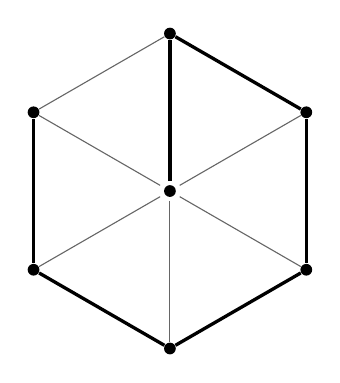
\begin{tikzpicture}
                    \graph  [nodes={circle,fill=black, empty nodes, inner sep=1.5pt}, edges={black!60, thin}, clockwise, radius=8em,
                    n=9, p=0.3] 
                    { subgraph C_n [n=6,m=3,clockwise,radius=2cm,name=A] };
                    \node at ($(A 1)!.5!(A 4)$) (C){};
                    \foreach \i in {1,2,...,6}{
                    \draw[black!60, thin] (C) -- (A \i); }
                    \node[circle, inner sep=1.5pt, fill=black] at (C) {};

                    % Thick path from center to 1
                    \draw [very thick] (C) -- (A 1);

                    % Thick path 1 to 2
                    \draw [very thick] (A 1) -- (A 2);

                    % Thick path 2 to 3
                    \draw [very thick] (A 2) -- (A 3);

                    % Thick path 3 to 4
                    \draw [very thick] (A 3) -- (A 4);

                    % Thick path 4 to 5
                    \draw [very thick] (A 4) -- (A 5);

                    % Thick path 5 to 6
                    \draw [very thick] (A 5) -- (A 6);
                \end{tikzpicture}
            \end{minipage}
            \begin{minipage}[b]{0.5\linewidth}
                \centering
                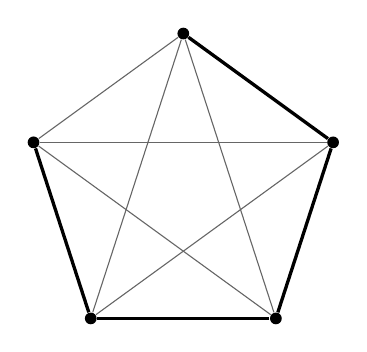
\begin{tikzpicture}
                    \graph  [nodes={circle,fill=black, empty nodes, inner sep=1.5pt}, edges={black!60, thin}, clockwise, radius=8em,
                    n=9, p=0.3] 
                    { subgraph K_n [n=5,clockwise,radius=2cm,name=A] };
                    
                    % Thick path from 1 to 2
                    \draw [very thick] (A 1) -- (A 2);

                    % Thick path 2 to 3
                    \draw [very thick] (A 2) -- (A 3);

                    % Thick path 3 to 4
                    \draw [very thick] (A 3) -- (A 4);

                    % Thick path 4 to 5
                    \draw [very thick] (A 4) -- (A 5);
                 \end{tikzpicture}
            \end{minipage}
            \begin{minipage}[b]{0.5\linewidth}
                \centering
                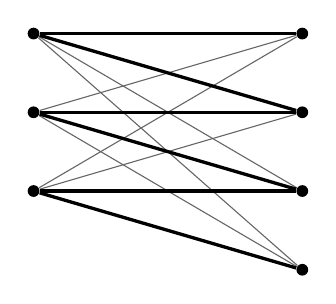
\begin{tikzpicture}
                    \graph[nodes={circle,fill=black, empty nodes, inner sep=1.5pt},edges={black!60, thin}, radius=8em, branch down=1 cm,
                    grow right sep=3.25cm] {subgraph I_nm [V={a,b,c}, W={1,...,4}];
                    a -- {1,2,3,4};
                    b -- {1,2,3,4};
                    c -- {1,2,3,4};
                    };           
                    
                    % Thick path from 1 to a
                    \draw [very thick] (1) -- (a);

                    % Thick path a to 2
                    \draw [very thick] (a) -- (2);

                    % Thick path 2 to b
                    \draw [very thick] (2) -- (b);

                    % Thick path b to 3
                    \draw [very thick] (b) -- (3);

                    % Thick path 3 to c
                    \draw [very thick] (3) -- (c);

                    % Thick path c to 4
                    \draw [very thick] (c) -- (4);
                \end{tikzpicture}
            \end{minipage}
            \begin{minipage}[b]{0.5\linewidth}
                \centering
                
\begin{tikzpicture}
                    \node[dot] (a) at (0,0) {};
                \end{tikzpicture}
            \end{minipage}
        \end{figure}
    \end{answer}

    % Question 5
    \begin{question}
        \label{q5}
        Prove Kruskal's Theorem.
    \end{question}

    % Answer 5
    \begin{answer}
        \label{a5}
    \end{answer}

    % Question 6
    \begin{question}
        \label{q6}
        Use Prim-Jarnik's or Kruskal's algorithm to find, step by step, the minimal spanning tree from the graph below. State what method you are using.
        \begin{figure}[H]
            \centering
            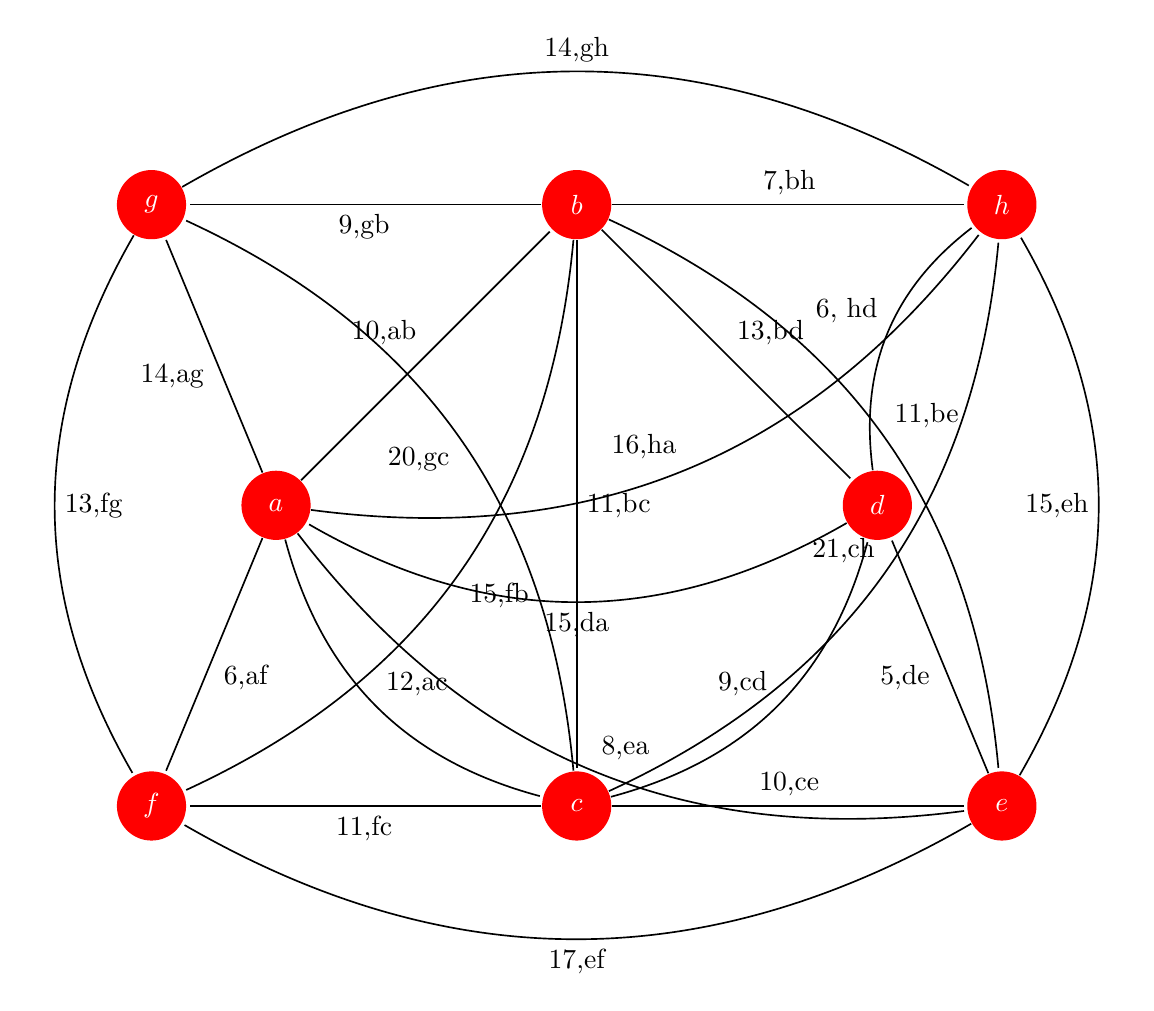
\begin{tikzpicture}[- ,shorten   >=1pt, auto, node distance=5.4cm, semithick]  %, >=stealth', 
                \tikzstyle{every state}=[fill=red,draw=none,text=white]
                \node[state] 	     (A)                             {$a$}; %initial,
                \node[state]         (B) [above right of=A] {$b$};
                \node[state]         (C) [below right of=A] {$c$};
                \node[state]         (D) [below right of=B] {$d$};
                \node[state]         (E) [right of= C]          {$e$};	
                \node[state]         (F) [ left of=C]          {$f$};
                \node[state]         (G) [left of=B]          {$g$};
                \node[state]         (H) [right of=B]          {$h$};
                \path (A) edge                 node  [auto] {10,ab} (B)
                              edge                [bend right]  node [auto] {12,ac} (C)
                             edge                node  [auto] {14,ag} (G)
                              edge               [bend right] node  [auto] {16,ha} (H)
                              edge              node [auto] {6,af} (F)
                              edge              [bend right] node [auto] {8,ea} (E)
              
                       (B)   edge          node  [auto] {11,bc} (C)
                               edge           node  [auto] {13,bd} (D)
                               edge          [bend left]           node  [auto]  {15,fb} (F)
                               edge            node   [auto] {9,gb} (G)
                               edge         [bend left]      node [auto] {11,be} (E)
                               edge              node [auto] {7,bh} (H)
                               
                          (C) edge        [bend right]    node [auto] {9,cd} (D)
                                edge               node [auto] {10,ce} (E)
                                edge              node [auto] {11,fc} (F)
                                edge        [bend right]       node [auto] {21,ch} (H)
                                edge        [bend right]       node  [auto]{20,gc} (G)
              
                       (E)   edge      [bend right]        node  [auto] {15,eh} (H)
                                          edge      [bend left]           node [auto] {17,ef } (F)
                              edge               		         node [auto] {5,de} (D)
                          
                      (G)   edge      [bend right]           node [auto] {13,fg} (F)
                                edge      [bend left]              node [auto]  {14,gh} (H)
                          
                          
                              (D)   edge       [bend left]         node [auto] {15,da} (A)
                                 edge          [bend left]        node [auto] {6, hd} (H);
              
              \end{tikzpicture}
        \end{figure}
    \end{question}

    % Answer 6
    \begin{answer}
        \label{a6}
    \end{answer}

    % Question 7
    \begin{question}
        \label{q7}
        Describe the tree produced by breadth-first search and depth-first search for the $n$-cube graph $Q_n$, where $n$ is a positive integer.
    \end{question}

    % Answer 7
    \begin{answer}
        \label{a7}
    \end{answer}

    % Question 8
    \begin{question}
        \label{q8}
        Build a binary search tree for the words: {\em oenology, phrenology, campanology, ornithology, ichthyology, limnology, alchemy,} and {\em astrology} using alphabetical order.   
     \end{question}

    % Answer 8
    \begin{answer}
        \label{a8}
    \end{answer}

    % Question 9
    \begin{question}
        \label{q9}
        For the tree in \hyperref[a8]{Question 8} determine the order in which a inorder traversal visits the vertices of the given ordered rooted tree.    
    \end{question}

    % Answer 9
    \begin{answer}
        \label{a9}
    \end{answer}

    % Question 10
    \begin{question}
        \label{q10}
        For the tree in \hyperref[a8]{Question 8} determine the order in which a postorder traversal visits the vertices of the given ordered rooted tree.
    \end{question}

    % Answer 10
    \begin{answer}
        \label{a10}
    \end{answer}

    % Question 11
    \begin{question}
        \label{q11}
        How many nonisomorphic unrooted trees are there with six vertices?
    \end{question}

    % Answer 11
    \begin{answer}
        \label{a11}
    \end{answer}

    % Question 12
    \begin{question}
        \label{q12}
        How many nonisomorphic rooted trees are there with six vertices    
    \end{question}

    % Answer 12
    \begin{answer}
        \label{a12}
    \end{answer}
\end{document} 
